% cloned from https://gitlab.kit.edu/kit/kastel/sdq/dokumentvorlagen/praesentationen/beamer
% commit: df83435a0d7e4308ba4115901166d32237c94d67

\documentclass[en, navbarinline, handout]{sdqbeamer}
% remove animation roll-out: handout (general "beamer" option, not specific for this class)
% layout options: 16:9 (default), 16:10, 4:3
% footer font size options: bigfoot (default), smallfoot (KIT layout)
% navigation bar options: navbarinline (default), navbarinfooter, navbarside, navbaroff, navbarkit (off + smallfoot)
% language: de (default), en

\titleimage{title_image}

\grouplogo{}

\groupname{PhD Defense}
%\groupnamewidth{50mm} % default

\title[Leveraging Constraints for User-Centric Feature Selection]{Leveraging Constraints for User-Centric Feature Selection} % [footer]{title slide}
\subtitle{PhD Defense}
\author[Jakob Bach]{Jakob Bach} % [footer]{title slide}

\date[2025-01-20]{January 20, 2025} % [footer]{title slide}

%\usepackage{amsmath} % mathematical symbols and equations; apparently pre-loaded
%\usepackage{amssymb} % mathematical symbols; apparently pre-loaded
\usepackage[style=numeric, backend=biber]{biblatex}
%\usepackage{graphicx} % plots; apparently pre-loaded
\usepackage{subcaption} % subfigures
%\usepackage{hyperref} % links and URLs; apparently pre-loaded

\addbibresource{references.bib}

\hypersetup{colorlinks=true, citecolor=kit-blue, linkcolor=kit-blue, urlcolor=kit-blue}

\setlength{\leftmargini}{0.2cm} % change default indentation (so items are left-aligned to boxes)
\setlength{\leftmarginii}{0.3cm} % 2nd level indentation
\setlength{\leftmarginiii}{0.3cm} % 3rd level indentation

\setbeamerfont{itemize/enumerate subsubbody}{size=\small} % make 3rd-level items as large as 2nd-level ones (default is \footnotesize, as defined in "beamerfontthemedefault.sty")

\setbeamercovered{invisible} % use "transparent" to show later content of animated slide in gray

\begin{document}

\KITtitleframe

\section{Introduction}

\begin{frame}[t]{Background and Motivation}
	\begin{definition}[Feature selection]
		Given a dataset~$X \in \mathbb{R}^{m \times n}$
		with prediction target~$y \in Y^m$ (e.g., $Y = \mathbb{R}$ or $Y = \{0, 1\}$),
		\emph{feature selection} is the problem of making feature-selection decisions~$s \in \{0,1\}^n$
		that maximize a given notion of feature-set quality~$Q(s,X,y)$.
		Typically, select a fixed number of features~$k \in \mathbb{N}$, i.e., $\sum_{j=1}^n s_j = k$.
	\end{definition}
	%JB: want to clarify which scenario we talk about
	%JB: very generally, we are in field of data science / machine learning
	%JB: focus on supervised feature selection for tabular data
	%JB: examples for prediction target from our experiments (though our methods are domain-independent): is person credit-worthy? is e-mail spam? is mushroom poisonous? will horse survive illness?
	%JB: feature engineering already done (e.g., in spam example)
	%JB: different white-box and black-box objectives for quality, depending on feature-selection method (from correlating each feature with the target to running a genetic algorithm wrapped around a prediction model)
	\pause
	\vspace{\baselineskip}
	\begin{itemize}
		\item Reasons for feature selection~\cite{chandrashekar2014survey, li2017feature}:
		\begin{itemize}
			\item Reduce computational requirements (CPU, memory, storage) of machine learning
			%JB: training and prediction
			\item Improve prediction performance
			% JB: IMHO questionable
			\item Increase interpretability of predictions
		\end{itemize}
		\pause
		\vspace{\baselineskip}
		\item Main limitations of most existing feature-selection methods:
		\begin{itemize}
			\item Do not consider domain knowledge
			%JB: Q() is a technical criterion, and there are typically no constraints apart from cardinality
			%JB: technically good feature sets may still be hard to interpret if they don't make sense from domain perspective
			%JB: domain knowledge may be firm, hypotheses, preferences
			%JB: in literature, there are at most approaches integrating specific constraint types into specific FS methods (apart from the work of Groves)
			\item Return only one feature set, no alternatives
			%JB: may be misleading if there are alternative solutions with similar quality
		\end{itemize}
	\end{itemize}
\end{frame}

\begin{frame}[t]{Approach}
	\begin{itemize}
		\item Central idea of dissertation: Make feature selection more user-centric via constraints
		%JB: we use constraints in propositional logic and linear arithmetic
		\begin{itemize}
			\item Still optimize feature-set quality but restrict valid feature selections
			\item Formulate as white-box optimization problem and use (MIP/SMT) solver
		\end{itemize}
		\pause
		%
		\begin{example}[A feature-selection constraint in propositional logic]
			$(\lnot s_1 \land \lnot s_2 \land \lnot s_3) \lor (s_1 \land s_2 \land s_3) \leftrightarrow$ ``Select none or all of Features 1, 2, and 3.''
		\end{example}
		%
		\pause
		\vspace{0.5\baselineskip}
		\item Benefits of our approach:
		\begin{itemize}
			\item Declarative
			\item Allows combining constraints
			\item Orthogonal to choice of feature-selection method
			%JB: related work typically integrates one constraint type into one feature-selection method
		\end{itemize}
	\end{itemize}
\end{frame}

\begin{frame}[t]{Contributions}
	\label{slide:contributions}
	\begin{itemize}
		\item Four core contributions of our dissertation:
		%JB: correspond to four chapters in main part
		\begin{itemize}
			\item (C1) Evaluating the impact of constraints \cite{bach2022empirical}
			\item (C2) Using constraints to formulate scientific hypotheses \cite{bach2022empirical}
			\item (C3) Using constraints for alternative feature sets \cite{bach2023finding, bach2024alternative}
			\item (C4) Using constraints for feature selection in subgroup discovery \cite{bach2025subgroup, bach2024using}
		\end{itemize}
		\item Sub-contributions like formalization, (complexity) analyses, and experimental studies
		%JB: presentation will focus on (C3) and (C4)
		\pause
		\vspace{\baselineskip}
		%JB: Meta-contibution:
		\item Reproducibility:
		\begin{itemize}
			\item All experimental data available on \href{https://doi.org/10.35097/4kjyeg0z2bxmr6eh}{RADAR4KIT}
			\item All code available:
			\begin{itemize}
				\item Three GitHub repositories [\href{https://github.com/Jakob-Bach/Constrained-Filter-Feature-Selection}{a}, \href{https://github.com/Jakob-Bach/Alternative-Feature-Selection}{b}, \href{https://github.com/Jakob-Bach/Constrained-Subgroup-Discovery}{c}]
				\item Three Python packages on PyPI: \href{https://pypi.org/project/alfese/}{\texttt{alfese}}, \href{https://pypi.org/project/cffs/}{\texttt{cffs}}, and \href{https://pypi.org/project/csd/}{\texttt{csd}}
			\end{itemize}
		\end{itemize}
	\end{itemize}
\end{frame}

\section{Constrained Feature Selection}

\begin{frame}[t]{(C1) Evaluating the Impacts of Constraints -- Approach}
	\begin{itemize}
		\item Systematic study on impact of constraints on feature-selection results
		\begin{itemize}
			\item Metrics for constraints, e.g, fraction of valid feature sets
			%JB: 4 metrics: number of constraints, number of (unique) constrained features, fraction of valid feature sets
			\item Metrics for results, e.g, feature-set quality
			%JB: 3 metrics: number of selected features, objective value, prediction performance
		\end{itemize}
		\pause
		\vspace{\baselineskip}
		\item Experimental design:
		\begin{itemize}
			\item 35 regression datasets from \emph{OpenML}~\cite{vanschoren2014openml}
			%JB: solution counting is expensive, therefore low dimensionality (10-14 features)
			%JB: 10-fold cross-validation
			\item Linear objective: $Q(s,X,y) = \sum_{j=1}^{n} q(X_{\cdot{}j},y) \cdot s_j$ (using mutual information~\cite{kraskov2004estimating} as $q(\cdot)$)
			%JB: very simple notion of feature-set quality (univariate filter)
			%JB: absolute Pearson correlation yielded similar insights
			%JB: also train four prediction models trained with selected features afterwards, but not in presented results: linear regression, regression tree, boosted linear model, boosted trees~\cite{chen2016xgboost, pedregosa2011scikit}
			\item Generate random constraints for ten constraint types with 1000 repetitions
			%JB: in each repetition, randomly choose features (for a varying number of constraints)
			%JB: unconstrained base case also is one of the constraint types
			\item \emph{Z3}~\cite{bjorner2015nuz, deMoura2008z3} (an SMT solver) as optimizer
		\end{itemize}
	\end{itemize}
	\pause
	\vspace{\baselineskip}
	\begin{examples}[Constraint types]
		\begin{itemize}
			\item $\text{Single-XOR}(s_{j_1}, s_{j_2}) = s_{j_1} \oplus s_{j_2} = (s_{j_1} \land \lnot s_{j_2}) \lor (\lnot s_{j_1} \land s_{j_2})$
			% JB; some constraints relate to only two features ("single"), some to a group of features ("group"), some to all ("global")
			\item $\text{Group-NAND}(\{s_{j_1}, \dots, s_{j_{n'}}\}) =	\lnot (s_{j_1} \land s_{j_2} \land \dots \land s_{j_{n'}}) = \sum_{l=1}^{n'} s_{j_l} \leq n'-1$
		\end{itemize}
	\end{examples}
\end{frame}

\begin{frame}[t]{(C1) Evaluating the Impacts of Constraints -- Results}
	\begin{figure}[htb]
		\centering
		\captionsetup{justification=centering}
		\begin{subfigure}{0.48\textwidth}
			\centering
			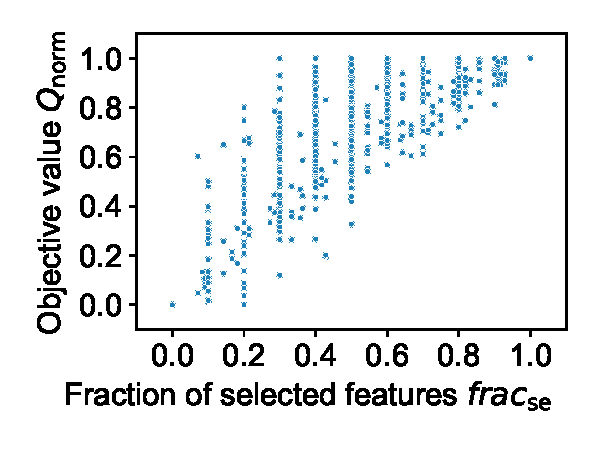
\includegraphics[width=\textwidth, trim={0 15 0 10}, clip]{plots/syn-selected-vs-objective.pdf}
			% \caption*{Fraction of selected features vs. normalized objective value.}
			%JB: all experimental results downsampled to 1000 random results to control plot file size
			%JB: normalization of number of selected features: divide by number of features in dataset
			%JB: normalization of objective value: divide by summed quality of all features of dataset
			%JB: clear correlation between number of selected features and objective (is expected)
		\end{subfigure}
		\hfill
		\begin{subfigure}{0.48\textwidth}
			\centering
			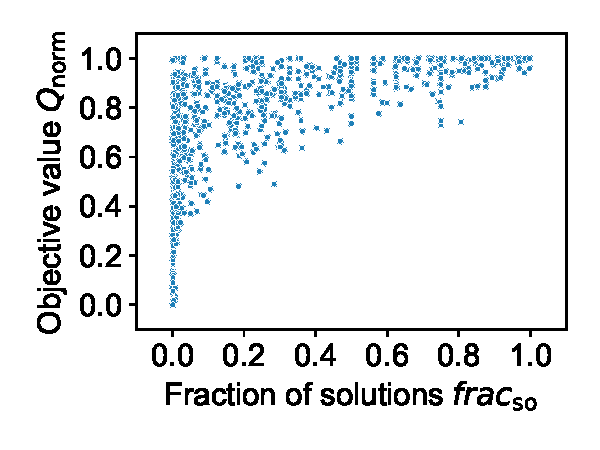
\includegraphics[width=\textwidth, trim={0 15 0 10}, clip]{plots/syn-solutions-vs-objective.pdf}
			% \caption*{Fraction of solutions vs. normalized objective value.}
			%JB: normalization of number of solutions: divide by total number of solutions (2 ^{number of features})
			%JB: clear correlation between size of solution space and objective (this trade-off is expected)
			%JB: even if solution space narrowed down significantly, high objective possible (the inverse does not hold)
			%JB: but existence of sweet spots naturally depends on dataset (how feature quality distributed)
			%JB: huge differences of individual evaluation metrics between constraint types
			%JB: weaker correlation if not taking size of solution space, but a cheaper proxy like number of constraints or number of constrained features
			%JB: note that we show objective of filter FS here; only weak to moderate correlation between number of solutions and prediction performance
		\end{subfigure}
	\end{figure}
\end{frame}

\section{Alternative Feature Selection}

\begin{frame}[t]{(C3) Finding Alternative Feature Sets}
	\begin{itemize}
		\item
	\end{itemize}
\end{frame}

\section{Constrained Subgroup Discovery}

\begin{frame}[t]{(C4) Finding Small and Alternative Subgroup Descriptions}
	\begin{itemize}
		\item
	\end{itemize}
\end{frame}

\section{Conclusion}

\begin{frame}[t]{Conclusions}
	\begin{itemize}
		\item Research gaps -- Most existing methods for feature selection and subgroup discovery:
		\begin{itemize}
			\item Do not consider domain knowledge
			\item Return only one solution, no alternatives
		\end{itemize}
		\pause
		\vspace{\baselineskip}
		\item Approach: Address both research gaps with constraints on selected feature sets
		\pause
		\vspace{\baselineskip}
		\item Core contributions:
		\begin{itemize}
			\item (C1) Evaluating the impact of constraints \cite{bach2022empirical}
			\item (C2) Using constraints to formulate scientific hypotheses \cite{bach2022empirical}
			\item (C3) Using constraints for alternative feature sets \cite{bach2023finding, bach2024alternative}
			\item (C4) Using constraints for feature selection in subgroup discovery \cite{bach2025subgroup, bach2024using}
		\end{itemize}
		\item All code and data available online
	\end{itemize}
\end{frame}

\appendix
\beginbackup % subsequent slides do not impact overall slide count

\begin{frame}[t, allowframebreaks]{References}
	\renewcommand*{\bibfont}{\small} % use a smaller font for bib than for main text
	\printbibliography
\end{frame}

\section{Appendix}

\begin{frame}[t]{Details of Underlying Publications}
	\begin{itemize}
		\item Constrained feature selection (\hyperlink{slide:contributions}{C1} and \hyperlink{slide:contributions}{C2}):
		\begin{itemize}
			\item \fullcite{bach2022empirical}
		\end{itemize}
		\item Alternative feature selection (\hyperlink{slide:contributions}{C3}):
		\begin{itemize}
			\item \fullcite{bach2023finding}
			\item \fullcite{bach2024alternative}
		\end{itemize}
		\item Constrained subgroup discovery (\hyperlink{slide:contributions}{C4}):
		\begin{itemize}
			\item \fullcite{bach2024using}
			\item \fullcite{bach2025subgroup}
		\end{itemize}
	\end{itemize}
\end{frame}

\begin{frame}[t]{Related Work}
	%JB: only small selection of related work discussed in dissertation
	\begin{itemize}
		\item Integrating domain knowledge and constraints:
		\begin{itemize}
			\item Feature selection: Typically only combination of one constraint type (like cost~\cite{paclik2002feature, plasberg2009feature}, cardinality~\cite{khushaba2011feature, yang2015budget}, or group~\cite{jacob2009group, yuan2006model}) and feature-selection method; exceptions (wrapper methods with black-box constraints):~\cite{groves2015toward, neutatz2021enforcing}
			%JB: Groves (2015) ignores invalid feature sets in four wrapper FS methods (no white-box solver), uses narrow set of constraint types (related to hierarchical feature grouping and temporal lags)
			%JB: Neutatz (2021) works with black-box constraints that mostly relate to whole ML system (acuuracy, fairness, training time, etc.) rather than feature selection per se (except number of selected features) and are checked after training/evaluation
			%JB: other notions of "constrained feature selection" include semi-supervised learning (constraints related to data objects) and Bayesian network learning (conditional independence constraints, learned and propagated automatically)
			\item Subgroup discovery: White-box formulations of different problem definitions~\cite{eckstein2002maximum, louveaux2014combinatorial} and integration of constraints into algorithmic search methods~\cite{atzmueller2005exploiting, meeng2021real}
			%JB: other white-box formulations use different constraint types, are CP or MIP (but not SMT), and do not compare against heuristics
			%JB: Maximum Box Problem (Eckstein 2002): capture as many positives as possible but no negatives
			%JB: Box Search Problem (Louveaux 2014): optimize sum of target variable of subgroup members (where target is continuous and can be negative)
			%JB: some SD methods use automatic quality-based pruning during search, but that approach differs from user constraints
			%JB: typical constraint types according to Meeng (2021): LB on quality, LB on members, UB on search depth
			%JB: studies on feature-cardinality constraint typically limited to one SD method or one cardinality threshold
			\item Other fields: E.g., AutoML~\cite{neutatz2023automl}, clustering~\cite{dao2024review}, pattern mining~\cite{silva2016constrained}, XAI~\cite{deutch2019constraints}; outside ML: software engineering~\cite{galindo2019automated}
			%JB: in ML, different problem definitions; software engineering has technically same problem as we (depending on objective function) but different domain/interpretation; technically, they often combine algorithm with sat solving, but pure white-box approach exist as well
		\end{itemize}
		\vspace{\baselineskip}
		\item Finding alternative solutions:
		\begin{itemize}
			\item Feature selection: Approaches that offer less user control over alternatives, e.g., ensemble feature selection~\cite{guru2018alternative, shekar2017diverse} or statistically equivalent feature sets~\cite{borboudakis2021extending, lagani2017feature}
			%JB: generally, less user control: in particular, no dissimilarity threshold
			%JB: ensemble feature selection: diversity may be sub-goal, but should "only" increase prediction performance in end (composition of feature sets is not of interest per se)
			%JB: statistically equivalent feature sets: no control over number, no redundancy at all, statistically equivalent for predictions, while we allow degradation of prediction performance and feature-set overlap (more flexible)
			\item Subgroup discovery: Subgroup-set selection~\cite{lucas2018ssdp+, proencca2022robust}; different problem definitions of alternative descriptions, e.g., description-based subgroup selection~\cite{leeuwen2012diverse} or equivalent subgroup descriptions of minimal length~\cite{boley2009non}
			%JB: subgroup-set selection wants to minimize rather than maximize overlap of data objects, and does not care about feature selection
			%JB: besides simultaneous search for diverse subgroups, also covering (exclude previously covered data objects), weighting, resampling, and post-processing approaches
			%JB: Leeuwen (2012) proposes 6 strategies for subgroup diversity, two related to descriptions, both integrated into simultaneous beam search, both offers less control than we do: (1) exclude descriptions with same quality and one condition less; (2) global bound on how often each feature selected in subgroup set
			%JB: Boley (2009): cover exactly same data objects with subset of given features; two search algorithms (not solver-based); inspired our NP-hardness proof
			\item Other fields: E.g., clustering~\cite{bailey2014alternative}, number partitioning~\cite{lawrinenko2017identical}, subspace search~\cite{fouche2021efficient}, XAI~\cite{mothilal2020explaining}
			%JB: problem definitions differ from ours (objective, constraints for alternatives)
			%JB: XAI example: counterfactuals should have different prediction outcome (rather than similar prediction quality) but similar feature values (rather than different feature selection)
		\end{itemize}
	\end{itemize}
\end{frame}

\begin{frame}[t]{Future Work}
	%JB: dissertation contains more ideas
	\begin{itemize}
		\item Different areas/directions: ML methodology, applied ML, and complexity theory
		%JB: results in one of these areas may be not that interesting for researchers from other areas
		\vspace{\baselineskip}
		\item ML methodology:
		\begin{itemize}
			\item Integrating constraints into more methods
			%JB: for FS, we focused on filter methods / white-box solving; only one wrapper, no embedded method
			\item Soft constraints
			%JB: may be violated; multi-objective problem, where solutions from Pareto front may be shown to user, or trade-off parameter
			\item Feature engineering
			%JB: could develop constraints for feature-creation operators, and/or consider constraint in automated feature engineering
		\end{itemize}
		\item Applied ML:
		\begin{itemize}
			\item Case studies with qualitative interpretation of results
			%JB: our interpretation is quantitative
			\item User-friendly systems
			%JB: we have Python packages (friendly for ML experts), but no interface for end users
		\end{itemize}
		\item Complexity theory:
		%JB: also further work regarding NP-hardness possible, e.g., objectives in AFS and feature-set overlap in ASDD
		\begin{itemize}
			\item Approximation complexity
			%JB: rather loose results (APX membership) for one quality function in AFS, no results in SD (though heuristic methods strong there as well)
			\item Parameterized complexity
			%JB: rather loose results at moment (XP membership), may be narrowed down
		\end{itemize}
	\end{itemize}
\end{frame}

\begin{frame}[t]{(C2) Scientific Hypotheses as Constraints -- Approach}
	\begin{itemize}
		\item Case study on impact of constraints in a specific use case
		\begin{itemize}
			\item Scenario~\cite{sudmanns2020data} from materials science: Predict density of dislocation reactions in a specimen under load
			%JB: Tensile test with aluminum specimen (could also be other face-centered cubic crystal)
			%JB: Dislocations (defects in material) appear and move as specimen deforms; reaction desnity should be predicted from other physical quantities
			%JB: Size of (5 micrometers)^3, partitioned into 5^3 voxels
			%JB: 22 time steps with intervals of ~ 5 ns
			\item Constraints express preferences regarding feature sets and hypotheses from domain
			%JB: preferences: global cardinality, inter-correlation, quality filter
			\item Idea: Hypotheses inconsistent to data should lower prediction quality significantly
		\end{itemize}
		\vspace{\baselineskip}
		\item Experimental design:
		\begin{itemize}
			\item One dataset with 14,903 data objects, 135 features, and continuous target
			\item Linear objective using Pearson correlation as $q(\cdot)$, four prediction models
			\item Constraint types: Three domain-independent (preferences) and twelve domain-specific (hypotheses)
		\end{itemize}
		\vspace{\baselineskip}
		\begin{example}[Constraint type]
			$\text{Aggregate-or-original}(\{s_1, \dots, s_n\}) = \bigwedge_{p \in P} \left( \left( \bigvee_{a \in A} s_{(p,a)} \right) + \left( \bigvee_{l \in \{1, \dots, 12\}} s_{(p,l)} \right) \leq 1 \right)$\\
			$\leftrightarrow$ ``For each physical quantity $p$, do not select aggregate features $a$ and original features $l$ at the same time.'' %JB: original features measured in 12 directions (slip systems)
		\end{example}
	\end{itemize}
\end{frame}

\begin{frame}[t]{(C2) Scientific Hypotheses as Constraints -- Results}
	\begin{figure}
		\centering
		\begin{subfigure}{0.48\textwidth}
			\centering
			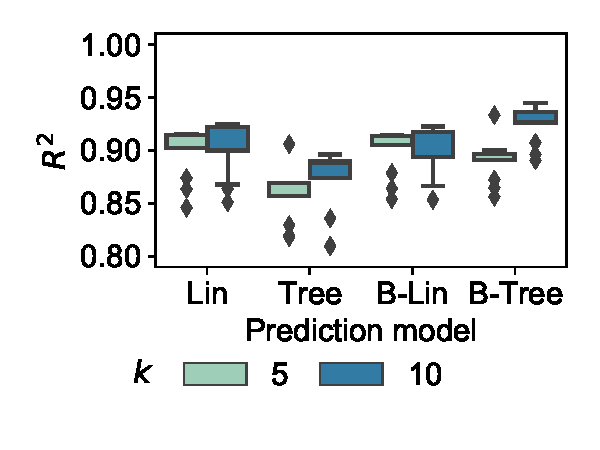
\includegraphics[width=\textwidth, trim={0 15 0 15}, clip]{plots/ms-prediction-performance-cardinality.pdf}
			\caption*{Distribution of prediction quality over constraint types (hypotheses).}
			%JB: performance for k=5 comparable to k=10, and even simple linear regression good (feature selection makes sense in scenario)
			%JB: not much difference of prediction performance between constraint types -> cannot invalidate hypotheses
			%JB: similar observations as for prediction performance also for objective value
		\end{subfigure}
		\hfill
		\begin{subfigure}{0.48\textwidth}
			\centering
			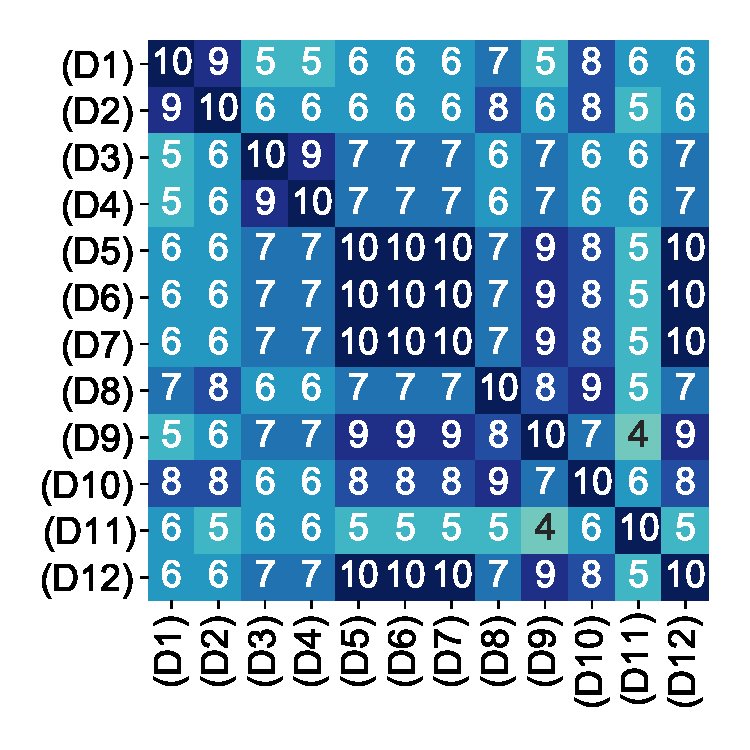
\includegraphics[width=0.7\textwidth, trim={0 15 0 15}, clip]{plots/ms-selected-similarity-card10.pdf}
			\caption*{Overlap size of feature sets between constraint types (for $k=10$).}
			%JB: event though prediction performance similar, feature sets might differ -> interesting alternatives
			%JB: still, quite often results similar to UNCONSTRAINED (D12) -> constraints might not affect top features or top feature set might already satisfy constraints -> iterating with domain experts probably better
			%JB: selected features made sense to domain experts, mostly related to dislocation density
		\end{subfigure}
	\end{figure}
\end{frame}

\backupend

\end{document}
